\section{ejercicio 2}
\par Sea $
f\left(x\right):=3\,\left(x+1\right)\,\left(x-\frac{1}{2}\right)\,\left(x-1\right)
$. Use el método de bisección para encontrar $p_3$ en los siguientes
intervalos.
\begin{itemize}
\item[a)] $[-2, 1.5]$
\item[b)] $[-1.25, 2.5]$
\end{itemize}

\subsection{inciso a)}
\begin{verbatim}
  $ biseccion(-2,1.5,5,3);
\end{verbatim}

\[
  \pmatrix{N&a&b&p&\mathrm{f}\left(a\right)&\mathrm{f}\left(b\right)&\mathrm{f}\left(p\right)&\mathrm{f}\left(a\right)
    * \mathrm{f}\left(p\right)&\mathrm{error}\cr
    1&-2&1.5&-0.25&-22.5&3.75&2.109375&-47.4609375&1.75\cr
    2&-2&-0.25&-1.125&-22.5&2.109375&-1.2949219&29.1357428&0.875\cr
    3&-1.125&-0.25&-0.6875&-1.2949219&2.109375&1.8786621&-2.4327207&0.4375\cr
  }
\]

\subsection{inciso b)}
\begin{verbatim}
  biseccion(-1.25,2.5,5,3);
\end{verbatim}

\[
  \pmatrix{N&a&b&p&\mathrm{f}\left(a\right)&\mathrm{f}\left(b\right)&\mathrm{f}\left(p\right)&\mathrm{f}\left(a\right)
    * \mathrm{f}\left(p\right)&\mathrm{error}\cr
    1&-1.25&2.5&0.625&-2.953125&31.5&-0.2285156&0.6748351&1.875\cr
    2&0.625&2.5&1.5625&-0.2285156&31.5&4.5944824&-1.0499109&0.9375\cr
    3&0.625&1.5625&1.09375&-0.2285156&4.5944824&0.3496399&-0.0798982&0.46875\cr
  }
\]

\section{ejercicio 3}
\par Use el método de biseccion para encontrar la solución de $
f\left(x\right):=x^3-7\,x^2+14\,x-6$ con una toleracia de $10^{-2}$

\subsection{inciso b)}
En el intervalo $[1,3.2]$

\begin{verbatim}
  f(x):=x^3-7*x^2+14*x-6;
  biseccion(1,3.2,2,20);
\end{verbatim}

$$
\pmatrix{N&a&b&p&f\left(a\right)&f\left(b\right)&f\left(p\right)&f
 \left(a\right)\,f\left(p\right)&{\it error}\cr 1&1&3.2&2.1&2&-0.112&
 1.791&3.582&1.1\cr 2&2.1&3.2&2.65&1.791&-0.112&0.552&0.989&0.55\cr 3
 &2.65&3.2&2.925&0.552&-0.112&0.0858&0.0474&0.275\cr 4&2.925&3.2&
 3.0625&0.0858&-0.112&-0.0544&-0.00467&0.137\cr 5&2.925&3.0625&2.9938
 &0.0858&-0.0544&0.00633&5.4311 \times 10^{-4}&0.0687\cr 6&2.9938&
 3.0625&3.0281&0.00633&-0.0544&-0.0265&-1.6782 \times 10^{-4}&0.0344
 \cr 7&2.9938&3.0281&3.0109&0.00633&-0.0265&-0.0107&-
 6.76889 \times 10^{-5}&0.0172\cr 8&2.9938&3.0109&3.0023&0.00633&-
 0.0107&-0.00233&-1.47614 \times 10^{-5}&0.00859\cr }
$$

\section{ejercicio 5}
\par Use el metodo de biseccion para encontrar la solución, de los
siguientes, con una tolerancia de $10^{-5}$

\subsection{inciso a)}
La funcion $f(x):=x-2^{-x}$ en el intervalo $[0,1]$

\begin{verbatim}
  f(x):=x-2^(-x);
  biseccion(0, 1, 5, 20);
\end{verbatim}

{\scriptsize
$$\pmatrix{N&a&b&p&f\left(a\right)&f\left(b\right)&f\left(p\right)&f
 \left(a\right)\,f\left(p\right)&{\it error}\cr 1&0&1&0.5&-1&0.5&-
 0.207107&0.207107&0.5\cr 2&0.5&1&0.75&-0.207107&0.5&0.155396&-
 0.0321837&0.25\cr 3&0.5&0.75&0.625&-0.207107&0.155396&-0.0234198&
 0.00485039&0.125\cr 4&0.625&0.75&0.6875&-0.0234198&0.155396&
 0.0665711&-0.00155908&0.0625\cr 5&0.625&0.6875&0.65625&-0.0234198&
 0.0665711&0.0217245&-5.08783454 \times 10^{-4}&0.03125\cr 6&0.625&
 0.65625&0.640625&-0.0234198&0.0217245&-8.10008039 \times 10^{-4}&
 1.89702079 \times 10^{-5}&0.015625\cr 7&0.640625&0.65625&0.648438&-
 8.10008039 \times 10^{-4}&0.0217245&0.0104666&-
 8.47803889 \times 10^{-6}&0.0078125\cr 8&0.640625&0.648438&0.644531&
 -8.10008039 \times 10^{-4}&0.0104666&0.00483065&-
 3.9128623 \times 10^{-6}&0.00390625\cr 9&0.640625&0.644531&0.642578&
 -8.10008039 \times 10^{-4}&0.00483065&0.00201091&-
 1.62885012 \times 10^{-6}&0.00195313\cr 10&0.640625&0.642578&
 0.641602&-8.10008039 \times 10^{-4}&0.00201091&
 6.00595889 \times 10^{-4}&-4.86487499 \times 10^{-7}&
 9.765625 \times 10^{-4}\cr 11&0.640625&0.641602&0.641113&-
 8.10008039 \times 10^{-4}&6.00595889 \times 10^{-4}&-
 1.0466935 \times 10^{-4}&8.47830146 \times 10^{-8}&
 4.8828125 \times 10^{-4}\cr 12&0.641113&0.641602&0.641357&-
 1.0466935 \times 10^{-4}&6.00595889 \times 10^{-4}&
 2.4797245 \times 10^{-4}&-2.5955115 \times 10^{-8}&
 2.44140625 \times 10^{-4}\cr 13&0.641113&0.641357&0.641235&-
 1.0466935 \times 10^{-4}&2.4797245 \times 10^{-4}&
 7.16538452 \times 10^{-5}&-7.49996137 \times 10^{-9}&
 1.22070313 \times 10^{-4}\cr 14&0.641113&0.641235&0.641174&-
 1.0466935 \times 10^{-4}&7.16538452 \times 10^{-5}&-
 1.65071784 \times 10^{-5}&1.72779562 \times 10^{-9}&
 6.10351563 \times 10^{-5}\cr 15&0.641174&0.641235&0.641205&-
 1.65071784 \times 10^{-5}&7.16538452 \times 10^{-5}&
 2.75734769 \times 10^{-5}&-4.55160301 \times 10^{-10}&
 3.05175781 \times 10^{-5}\cr 16&0.641174&0.641205&0.64119&-
 1.65071784 \times 10^{-5}&2.75734769 \times 10^{-5}&
 5.5331851 \times 10^{-6}&-9.13372735 \times 10^{-11}&
 1.52587891 \times 10^{-5}\cr 17&0.641174&0.64119&0.641182&-
 1.65071784 \times 10^{-5}&5.5331851 \times 10^{-6}&-
 5.48698768 \times 10^{-6}&9.05746843 \times 10^{-11}&
 7.62939453 \times 10^{-6}\cr }$$
}

\subsection{inciso c)}
\par En el intervalo $[-3, -2]$ y $[-1, 0]$ con la funcion $
f\left(x\right):=2\,x\,\cos
\left(2\,x\right)-\left(x+1\right)^2$

\subsubsection{intervalo [-3, -2]}

\begin{verbatim}
  f(x):=2*x*cos(2*x)-(x+1)^2;
  biseccion(-3, -2, 5, 20);
\end{verbatim}


{\tiny
$$\pmatrix{N&a&b&p&f\left(a\right)&f\left(b\right)&f\left(p\right)&f
 \left(a\right)\,f\left(p\right)&{\it error}\cr 1&-3&-2&-2.5&-
 9.7610217&1.6145745&-3.6683109&35.806463&0.5\cr 2&-2.5&-2&-2.25&-
 3.6683109&1.6145745&-0.613919&2.2520454&0.25\cr 3&-2.25&-2&-2.125&-
 0.613919&1.6145745&0.630247&-0.38692&0.125\cr 4&-2.25&-2.125&-2.1875
 &-0.613919&0.630247&0.0380755&-0.0233753&0.0625\cr 5&-2.25&-2.1875&-
 2.21875&-0.613919&0.0380755&-0.280836&0.172411&0.03125\cr 6&-2.21875
 &-2.1875&-2.203125&-0.280836&0.0380755&-0.119557&0.0335759&0.015625
 \cr 7&-2.203125&-2.1875&-2.1953125&-0.119557&0.0380755&-0.0402785&
 0.00481557&0.0078125\cr 8&-2.1953125&-2.1875&-2.1914063&-0.0402785&
 0.0380755&-9.85194952 \times 10^{-4}&3.96821888 \times 10^{-5}&
 0.00390625\cr 9&-2.1914063&-2.1875&-2.1894531&-
 9.85194952 \times 10^{-4}&0.0380755&0.0185743&-
 1.8299343 \times 10^{-5}&0.00195313\cr 10&-2.1914063&-2.1894531&-
 2.1904297&-9.85194952 \times 10^{-4}&0.0185743&0.00880185&-
 8.67153955 \times 10^{-6}&9.765625 \times 10^{-4}\cr 11&-2.1914063&-
 2.1904297&-2.190918&-9.85194952 \times 10^{-4}&0.00880185&0.00391015
 &-3.85225692 \times 10^{-6}&4.8828125 \times 10^{-4}\cr 12&-
 2.1914063&-2.190918&-2.1911621&-9.85194952 \times 10^{-4}&0.00391015
 &0.00146293&-1.44127166 \times 10^{-6}&2.44140625 \times 10^{-4}\cr 
 13&-2.1914063&-2.1911621&-2.1912842&-9.85194952 \times 10^{-4}&
 0.00146293&2.38981324 \times 10^{-4}&-2.35443194 \times 10^{-7}&
 1.22070313 \times 10^{-4}\cr 14&-2.1914063&-2.1912842&-2.1913452&-
 9.85194952 \times 10^{-4}&2.38981324 \times 10^{-4}&-
 3.73078418 \times 10^{-4}&3.67554975 \times 10^{-7}&
 6.10351563 \times 10^{-5}\cr 15&-2.1913452&-2.1912842&-2.1913147&-
 3.73078418 \times 10^{-4}&2.38981324 \times 10^{-4}&-
 6.70414481 \times 10^{-5}&2.50117174 \times 10^{-8}&
 3.05175781 \times 10^{-5}\cr 16&-2.1913147&-2.1912842&-2.1912994&-
 6.70414481 \times 10^{-5}&2.38981324 \times 10^{-4}&
 8.59717127 \times 10^{-5}&-5.76366811 \times 10^{-9}&
 1.52587891 \times 10^{-5}\cr 17&-2.1913147&-2.1912994&-2.1913071&-
 6.70414481 \times 10^{-5}&8.59717127 \times 10^{-5}&
 9.46557602 \times 10^{-6}&-6.34585923 \times 10^{-10}&
 7.62939453 \times 10^{-6}\cr }$$
}

\subsubsection{intervalo [-1, 0]}

\begin{verbatim}
  f(x):=2*x*cos(2*x)-(x+1)^2;
  biseccion(-1, 0, 5, 20);
\end{verbatim}


{\tiny
$$\pmatrix{N&a&b&p&f\left(a\right)&f\left(b\right)&f\left(p\right)&f
 \left(a\right)\,f\left(p\right)&{\it error}\cr 1&-1&0&-0.5&0.832294&
 -1&-0.790302&-0.657764&0.5\cr 2&-1&-0.5&-0.75&0.832294&-0.790302&-
 0.168606&-0.14033&0.25\cr 3&-1&-0.75&-0.875&0.832294&-0.168606&
 0.296306&0.246613&0.125\cr 4&-0.875&-0.75&-0.8125&0.296306&-0.168606
 &0.0528816&0.0156691&0.0625\cr 5&-0.8125&-0.75&-0.78125&0.0528816&-
 0.168606&-0.0608144&-0.00321596&0.03125\cr 6&-0.8125&-0.78125&-
 0.796875&0.0528816&-0.0608144&-0.00468056&-2.47515541 \times 10^{-4}
 &0.015625\cr 7&-0.8125&-0.796875&-0.804688&0.0528816&-0.00468056&
 0.0239252&0.0012652&0.0078125\cr 8&-0.804688&-0.796875&-0.800781&
 0.0239252&-0.00468056&0.00957807&2.29156947 \times 10^{-4}&
 0.00390625\cr 9&-0.800781&-0.796875&-0.798828&0.00957807&-0.00468056
 &0.00243764&2.33478872 \times 10^{-5}&0.00195313\cr 10&-0.798828&-
 0.796875&-0.797852&0.00243764&-0.00468056&-0.00112424&-
 2.74050365 \times 10^{-6}&9.765625 \times 10^{-4}\cr 11&-0.798828&-
 0.797852&-0.79834&0.00243764&-0.00112424&6.56003277 \times 10^{-4}&
 1.59910056 \times 10^{-6}&4.8828125 \times 10^{-4}\cr 12&-0.79834&-
 0.797852&-0.798096&6.56003277 \times 10^{-4}&-0.00112424&-
 2.34294318 \times 10^{-4}&-1.5369784 \times 10^{-7}&
 2.44140625 \times 10^{-4}\cr 13&-0.79834&-0.798096&-0.798218&
 6.56003277 \times 10^{-4}&-2.34294318 \times 10^{-4}&
 2.10811015 \times 10^{-4}&1.38292717 \times 10^{-7}&
 1.22070313 \times 10^{-4}\cr 14&-0.798218&-0.798096&-0.798157&
 2.10811015 \times 10^{-4}&-2.34294318 \times 10^{-4}&-
 1.17525187 \times 10^{-5}&-2.47756039 \times 10^{-9}&
 6.10351563 \times 10^{-5}\cr 15&-0.798218&-0.798157&-0.798187&
 2.10811015 \times 10^{-4}&-1.17525187 \times 10^{-5}&
 9.95265316 \times 10^{-5}&2.09812892 \times 10^{-8}&
 3.05175781 \times 10^{-5}\cr 16&-0.798187&-0.798157&-0.798172&
 9.95265316 \times 10^{-5}&-1.17525187 \times 10^{-5}&
 4.38863273 \times 10^{-5}&4.36785394 \times 10^{-9}&
 1.52587891 \times 10^{-5}\cr 17&-0.798172&-0.798157&-0.798164&
 4.38863273 \times 10^{-5}&-1.17525187 \times 10^{-5}&
 1.60667345 \times 10^{-5}&7.05109969 \times 10^{-10}&
 7.62939453 \times 10^{-6}\cr }$$
}

\section{ejercicio 7}

\subsection{inciso a)}
Grafique $y=x$ y $y=2*sin(x)$ en un mismo cuadro.

\begin{verbatim}
  wxplot2d([x,2*sin(x)],[x,-5,5]);
\end{verbatim}

\begin{figure}[H]
  \centering
  \includegraphics[scale=0.45]{img/maxout_1.eps}
\end{figure}

\subsection{inciso b)}
\begin{verbatim}
  f(x):=2*sin(x);
  biseccion(3.05, 3.2, 5, 20);
\end{verbatim}

{\scriptsize
$$\pmatrix{N&a&b&p&f\left(a\right)&f\left(b\right)&f\left(p\right)&f
 \left(a\right)\,f\left(p\right)&{\it error}\cr 1&3.05&3.2&3.125&
 0.182929&-0.116748&0.0331838&0.00607029&0.075\cr 2&3.125&3.2&3.1625&
 0.0331838&-0.116748&-0.0418116&-0.00138747&0.0375\cr 3&3.125&3.1625&
 3.14375&0.0331838&-0.0418116&-0.00431469&-1.43177725 \times 10^{-4}&
 0.01875\cr 4&3.125&3.14375&3.134375&0.0331838&-0.00431469&0.0144352&
 4.79013963 \times 10^{-4}&0.009375\cr 5&3.134375&3.14375&3.1390625&
 0.0144352&-0.00431469&0.0050603&7.30463764 \times 10^{-5}&0.0046875
 \cr 6&3.1390625&3.14375&3.1414062&0.0050603&-0.00431469&
 3.72807177 \times 10^{-4}&1.88651682 \times 10^{-6}&0.00234375\cr 7&
 3.1414062&3.14375&3.1425781&3.72807177 \times 10^{-4}&-0.00431469&-
 0.00197094&-7.34781511 \times 10^{-7}&0.00117188\cr 8&3.1414062&
 3.1425781&3.1419922&3.72807177 \times 10^{-4}&-0.00197094&-
 7.99067799 \times 10^{-4}&-2.97898211 \times 10^{-7}&
 5.859375 \times 10^{-4}\cr 9&3.1414062&3.1419922&3.1416992&
 3.72807177 \times 10^{-4}&-7.99067799 \times 10^{-4}&-
 2.1313032 \times 10^{-4}&-7.9456513 \times 10^{-8}&
 2.9296875 \times 10^{-4}\cr 10&3.1414062&3.1416992&3.1415527&
 3.72807177 \times 10^{-4}&-2.1313032 \times 10^{-4}&
 7.98384296 \times 10^{-5}&2.97643396 \times 10^{-8}&
 1.46484375 \times 10^{-4}\cr 11&3.1415527&3.1416992&3.141626&
 7.98384296 \times 10^{-5}&-2.1313032 \times 10^{-4}&-
 6.66459454 \times 10^{-5}&-5.32090762 \times 10^{-9}&
 7.32421875 \times 10^{-5}\cr 12&3.1415527&3.141626&3.1415894&
 7.98384296 \times 10^{-5}&-6.66459454 \times 10^{-5}&
 6.59624209 \times 10^{-6}&5.26633609 \times 10^{-10}&
 3.66210937 \times 10^{-5}\cr 13&3.1415894&3.141626&3.1416077&
 6.59624209 \times 10^{-6}&-6.66459454 \times 10^{-5}&-
 3.00248517 \times 10^{-5}&-1.9805119 \times 10^{-10}&
 1.83105469 \times 10^{-5}\cr 14&3.1415894&3.1416077&3.1415985&
 6.59624209 \times 10^{-6}&-3.00248517 \times 10^{-5}&-
 1.17143048 \times 10^{-5}&-7.72703903 \times 10^{-11}&
 9.15527344 \times 10^{-6}\cr }$$
}

\section{ejercicio 9}

\subsection{inciso a)}
Grafique $y=e^x-2$ y $y=cos(e-2)$ en un mismo cuadro

\begin{verbatim}
  wxplot2d([%e^x-2,cos(%e^x-2)],[x,0,3]);
\end{verbatim}

\begin{figure}[H]
  \centering
  \includegraphics[scale=0.45]{img/maxout_3.eps}
\end{figure}


\subsection{inciso b)}
Use el método de biseccion para aproximar la intersección
$e^x-2=\cos\left(e-2\right)$ en el intervalo $[0.5, 1.5]$ con una
tolerancia $10^{-5}$

\begin{verbatim}
  f(x):=cos(%e-2)-%e^x+2;
  biseccion(0.5, 1.5, 5, 20);
\end{verbatim}


{\tiny
$$\pmatrix{N&a&b&p&f\left(a\right)&f\left(b\right)&f\left(p\right)&f
 \left(a\right)\,f\left(p\right)&{\it error}\cr 1&0.5&1.5&1.0&
 1.1042163&-1.7287515&0.0346557&0.0382674&0.5\cr 2&1.0&1.5&1.25&
 0.0346557&-1.7287515&-0.737405&-0.0255553&0.25\cr 3&1.0&1.25&1.125&
 0.0346557&-0.737405&-0.327279&-0.0113421&0.125\cr 4&1.0&1.125&1.0625
 &0.0346557&-0.327279&-0.140658&-0.00487462&0.0625\cr 5&1.0&1.0625&
 1.03125&0.0346557&-0.140658&-0.0516318&-0.00178934&0.03125\cr 6&1.0&
 1.03125&1.015625&0.0346557&-0.0516318&-0.00815098&-
 2.82478261 \times 10^{-4}&0.015625\cr 7&1.0&1.015625&1.0078125&
 0.0346557&-0.00815098&0.013336&4.62167997 \times 10^{-4}&0.0078125
 \cr 8&1.0078125&1.015625&1.0117188&0.013336&-0.00815098&0.00261348&
 3.48533162 \times 10^{-5}&0.00390625\cr 9&1.0117188&1.015625&
 1.0136719&0.00261348&-0.00815098&-0.0027635&-
 7.22234146 \times 10^{-6}&0.00195313\cr 10&1.0117188&1.0136719&
 1.0126953&0.00261348&-0.0027635&-7.36948619 \times 10^{-5}&-
 1.92600075 \times 10^{-7}&9.765625 \times 10^{-4}\cr 11&1.0117188&
 1.0126953&1.012207&0.00261348&-7.36948619 \times 10^{-5}&0.00127022&
 3.31969708 \times 10^{-6}&4.8828125 \times 10^{-4}\cr 12&1.012207&
 1.0126953&1.0124512&0.00127022&-7.36948619 \times 10^{-5}&
 5.98344986 \times 10^{-4}&7.60030235 \times 10^{-7}&
 2.44140625 \times 10^{-4}\cr 13&1.0124512&1.0126953&1.0125732&
 5.98344986 \times 10^{-4}&-7.36948619 \times 10^{-5}&
 2.62345571 \times 10^{-4}&1.56973157 \times 10^{-7}&
 1.22070313 \times 10^{-4}\cr 14&1.0125732&1.0126953&1.0126343&
 2.62345571 \times 10^{-4}&-7.36948619 \times 10^{-5}&
 9.43304821 \times 10^{-5}&2.47471842 \times 10^{-8}&
 6.10351563 \times 10^{-5}\cr 15&1.0126343&1.0126953&1.0126648&
 9.43304821 \times 10^{-5}&-7.36948619 \times 10^{-5}&
 1.0319092 \times 10^{-5}&9.73404922 \times 10^{-10}&
 3.05175781 \times 10^{-5}\cr 16&1.0126648&1.0126953&1.0126801&
 1.0319092 \times 10^{-5}&-7.36948619 \times 10^{-5}&-
 3.16875645 \times 10^{-5}&-3.26986893 \times 10^{-10}&
 1.52587891 \times 10^{-5}\cr 17&1.0126648&1.0126801&1.0126724&
 1.0319092 \times 10^{-5}&-3.16875645 \times 10^{-5}&-
 1.06841561 \times 10^{-5}&-1.1025079 \times 10^{-10}&
 7.62939453 \times 10^{-6}\cr }$$
}

\section{ejercicio 11}

\subsection{inciso b)}
Sea $f\left(x\right):=\left(x+2\right)\,\left(x+1\right)\,x\,\left(x-2\right)\,\left(x-1\right)^3$. Encuentre el cero de $f$ por el método de bisección.

\begin{verbatim}
  f(x):=(x+2)*(x+1)*x*(x-2)*(x-1)^3;
  biseccion(-2.5,3,3,20);
\end{verbatim}

{\small
$$\pmatrix{N&a&b&p&f\left(a\right)&f\left(b\right)&f\left(p\right)&f
 \left(a\right)\,f\left(p\right)&{\it error}\cr 1&-2.5&3&0.25&-
 361.758&480&0.5191&-187.79&2.75\cr 2&-2.5&0.25&-1.125&-361.758&
 0.5191&3.68975&-1334.8&1.375\cr 3&-2.5&-1.125&-1.8125&-361.758&
 3.68975&23.4202&-8472.43&0.6875\cr 4&-2.5&-1.8125&-2.15625&-361.758&
 23.4202&-50.9081&18416.4&0.3438\cr 5&-2.15625&-1.8125&-1.98438&-
 50.9081&23.4202&3.2324&-164.555&0.1719\cr 6&-2.15625&-1.98438&-
 2.07031&-50.9081&3.2324&-18.355&934.418&0.08594\cr 7&-2.07031&-
 1.98438&-2.02734&-18.355&3.2324&-6.36363&116.805&0.04297\cr 8&-
 2.02734&-1.98438&-2.00586&-6.36363&3.2324&-1.28615&8.18457&0.02148
 \cr 9&-2.00586&-1.98438&-1.99512&-1.28615&3.2324&1.0406&-1.33836&
 0.01074\cr 10&-2.00586&-1.99512&-2.00049&-1.28615&1.0406&-0.1056&
 0.1358&0.005371\cr 11&-2.00049&-1.99512&-1.9978&-0.1056&1.0406&
 0.4717&-0.04982&0.002686\cr 12&-2.00049&-1.9978&-1.99915&-0.1056&
 0.4717&0.1841&-0.01945&0.001343\cr 13&-2.00049&-1.99915&-1.99982&-
 0.1056&0.1841&0.03953&-0.004175&6.713867 \times 10^{-4}\cr }$$
}


\section{ejercicio 13}
Encuentre una aproximación de $\sqrt[3]{25}$ con una tolerancia de 
$10^{-4}$ por el método de bisección.

\begin{verbatim}
  f(x):=1-(25^(1/3)/x);
  biseccion(2.8, 3, 4, 20);
\end{verbatim}

{\scriptsize
$$\pmatrix{N&a&b&p&f\left(a\right)&f\left(b\right)&f\left(p\right)&f
 \left(a\right)\,f\left(p\right)&{\it error}\cr 1&2.8&3&2.9&-0.044292
 &0.025327&-0.008282&3.6682581 \times 10^{-4}&0.1\cr 2&2.9&3&2.95&-
 0.008282&0.025327&0.0088075&-7.2943911 \times 10^{-5}&0.05\cr 3&2.9&
 2.95&2.925&-0.008282&0.0088075&3.35816 \times 10^{-4}&-
 2.7812209 \times 10^{-6}&0.025\cr 4&2.9&2.925&2.9125&-0.008282&
 3.35816 \times 10^{-4}&-0.0039546&3.2751815 \times 10^{-5}&0.0125
 \cr 5&2.9125&2.925&2.91875&-0.0039546&3.35816 \times 10^{-4}&-
 0.0018048&7.1372113 \times 10^{-6}&0.00625\cr 6&2.91875&2.925&
 2.921875&-0.0018048&3.35816 \times 10^{-4}&-7.3334356 \times 10^{-4}
 &1.323533 \times 10^{-6}&0.003125\cr 7&2.921875&2.925&2.923437&-
 7.3334356 \times 10^{-4}&3.35816 \times 10^{-4}&-
 1.9847806 \times 10^{-4}&1.4555261 \times 10^{-7}&0.0015625\cr 8&
 2.923437&2.925&2.924219&-1.9847806 \times 10^{-4}&
 3.35816 \times 10^{-4}&6.8740339 \times 10^{-5}&-
 1.3643449 \times 10^{-8}&7.8125 \times 10^{-4}\cr 9&2.923437&
 2.924219&2.923828&-1.9847806 \times 10^{-4}&6.8740339 \times 10^{-5}
 &-6.4851012 \times 10^{-5}&1.2871503 \times 10^{-8}&
 3.90625 \times 10^{-4}\cr 10&2.923828&2.924219&2.924023&-
 6.4851012 \times 10^{-5}&6.8740339 \times 10^{-5}&
 1.949125 \times 10^{-6}&-1.2640273 \times 10^{-10}&
 1.953125 \times 10^{-4}\cr 11&2.923828&2.924023&2.923926&-
 6.4851012 \times 10^{-5}&1.949125 \times 10^{-6}&-
 3.1449828 \times 10^{-5}&2.0395532 \times 10^{-9}&
 9.765625 \times 10^{-5}\cr }$$
}


\section{ejercicio 15}
Aproxime la solución de $f\left(x\right):=x^3-x-1$ en el intervalo $[1, 2]$
con una tolerancia de $10^{-4}$.

\begin{verbatim}
  f(x):=x^3-x-1;
  biseccion(1,2,4,20);
\end{verbatim}



{\scriptsize
$$\pmatrix{N&a&b&p&f\left(a\right)&f\left(b\right)&f\left(p\right)&f
 \left(a\right)\,f\left(p\right)&{\it error}\cr 1&1&2&1.5&-1&5&0.875&
 -0.875&0.5\cr 2&1&1.5&1.25&-1&0.875&-0.29688&0.29688&0.25\cr 3&1.25&
 1.5&1.375&-0.29688&0.875&0.22461&-0.066681&0.125\cr 4&1.25&1.375&
 1.3125&-0.29688&0.22461&-0.051514&0.015293&0.0625\cr 5&1.3125&1.375&
 1.34375&-0.051514&0.22461&0.082611&-0.0042556&0.03125\cr 6&1.3125&
 1.34375&1.328125&-0.051514&0.082611&0.014576&-
 7.5086113 \times 10^{-4}&0.015625\cr 7&1.3125&1.328125&1.320313&-
 0.051514&0.014576&-0.018711&9.6385239 \times 10^{-4}&0.0078125\cr 8&
 1.320313&1.328125&1.324219&-0.018711&0.014576&-0.0021279&
 3.9815164 \times 10^{-5}&0.0039063\cr 9&1.324219&1.328125&1.326172&-
 0.0021279&0.014576&0.0062088&-1.321205 \times 10^{-5}&0.0019531\cr 
 10&1.324219&1.326172&1.325195&-0.0021279&0.0062088&0.0020367&-
 4.3338815 \times 10^{-6}&9.765625 \times 10^{-4}\cr 11&1.324219&
 1.325195&1.324707&-0.0021279&0.0020367&-4.6594883 \times 10^{-5}&
 9.9151369 \times 10^{-8}&4.8828125 \times 10^{-4}\cr 12&1.324707&
 1.325195&1.324951&-4.6594883 \times 10^{-5}&0.0020367&
 9.9479097 \times 10^{-4}&-4.6352169 \times 10^{-8}&
 2.4414063 \times 10^{-4}\cr 13&1.324707&1.324951&1.324829&-
 4.6594883 \times 10^{-5}&9.9479097 \times 10^{-4}&
 4.7403882 \times 10^{-4}&-2.2087783 \times 10^{-8}&
 1.2207031 \times 10^{-4}\cr 14&1.324707&1.324829&1.324768&-
 4.6594883 \times 10^{-5}&4.7403882 \times 10^{-4}&
 2.1370716 \times 10^{-4}&-9.9576603 \times 10^{-9}&
 6.1035156 \times 10^{-5}\cr }$$
}

\section{ejercicio 19)}
Un tanque de longitud $L$ tiene una seccion transversal semicircular
de radio $r$. El agua a una distancia $h$ de la parte superior tiene
un volumen $V$
\[
  V=L[0.5\,\pi\,r^2-r^2\,arcsin(h/r)-h\,(r^2-h^2)^{1/2}]
\]

\begin{figure}[H]
  \centering
  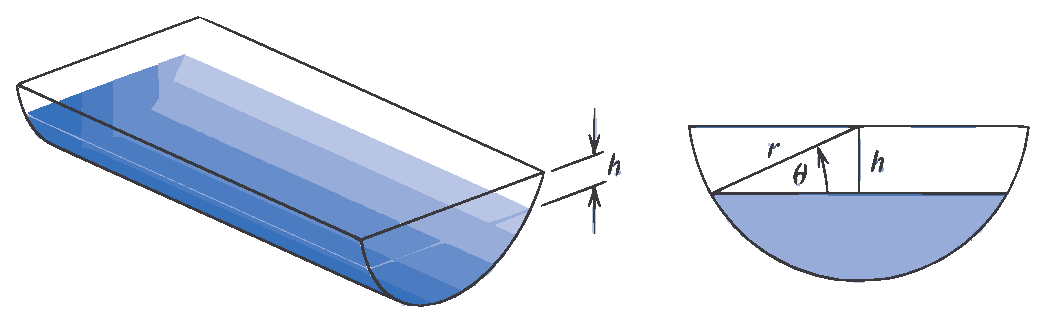
\includegraphics[scale=0.6]{img/tanque.eps}
\end{figure}

Suponga que $L=10\,ft$, $r=1\,ft$, y $V=12.4\,ft^3$. Encuentre la
\textbf{profundidad} del agua en el tanque con una tolerancia de $0.01\,ft$.
\begin{eqnarray} 
12.4 &=&10\,[0.5\,\pi\,1^2-1^2\,arcsin(h/1)-h\,(1^2-h^2)^{1/2}] \nonumber\\
12.4 &=&10\,[0.5\,\pi\,-arcsin(h)-h\,(1-h^2)^{1/2}] \nonumber
\end{eqnarray}

\par se necesita un $h$ tal que al sustituir en el miembro derecho de
$12.4$. Si se resta $12.4$ a la ecuación se tiene
\[
  0=10\,[0.5\,\pi\,-arcsin(h)-h\,(1-h^2)^{1/2}]-12.4
\]

\par luego se require un $h$, tal que al sustituir, de el valor de
$0$. En otras palabras, es menester hallar la raíz de la funcion, que
ahora lo definimos como $f\left(h\right)$
\[
  f\left(h\right)=10\,[0.5\,\pi\,-arcsin(h)-h\,(1-h^2)^{1/2}]-12.4=0
\]

\begin{verbatim}
  f(h):=10*(0.5*%pi-asin(h)-h*(1-h^2)^(1/2))-12.4;
  biseccion(0,1,3,20);
\end{verbatim}

$$\pmatrix{N&a&b&p&f\left(a\right)&f\left(b\right)&f\left(p\right)&f
 \left(a\right)\,f\left(p\right)&{\it error}\cr 1&0&1&0.5&3.30796&-
 12.4&-6.25815&-20.7017&0.5\cr 2&0&0.5&0.25&3.30796&-6.25815&-1.63945
 &-5.42325&0.25\cr 3&0&0.25&0.125&3.30796&-1.63945&0.8145&2.6943&
 0.125\cr 4&0.125&0.25&0.1875&0.8145&-1.63945&-0.4199&-0.342&0.0625
 \cr 5&0.125&0.1875&0.1563&0.8145&-0.4199&0.1957&0.1594&0.03125\cr 6&
 0.1563&0.1875&0.1719&0.1957&-0.4199&-0.1125&-0.02203&0.01563\cr 7&
 0.1563&0.1719&0.1641&0.1957&-0.1125&0.04149&0.008121&0.007813\cr 8&
 0.1641&0.1719&0.168&0.04149&-0.1125&-0.03555&-0.001475&0.003906\cr 9
 &0.1641&0.168&0.166&0.04149&-0.03555&0.002966&1.23086 \times 10^{-4}
 &0.001953\cr 10&0.166&0.168&0.167&0.002966&-0.03555&-0.01629&-
 4.832935 \times 10^{-5}&9.765625 \times 10^{-4}\cr }$$

por lo tanto $h=0.167$. Luego la profundidad es: radio menos el
valor de $h$ hallado
\[
  profundidad=r-h=1-0.167=0.833
\]

%%% Local Variables:
%%% TeX-master: "tarea1"
%%% End:
